\documentclass[10pt,a4paper]{article}
\usepackage[utf8]{inputenc}
\usepackage[english]{babel}
\usepackage{amsmath}
\usepackage{amsfonts}
\usepackage{amssymb}
\usepackage{setspace}
\usepackage[pdftex]{graphicx}
\usepackage{url}
\usepackage{listings}
\usepackage{nameref}


\usepackage[round]{natbib}
\usepackage{bibentry}
\nobibliography*

\begin{document}
\pagenumbering{gobble} % switch off page numbering
\onehalfspacing 
\begin{titlepage}
\author{Michael Jungo\footnote{michael.jungo@unifr.ch} \\ 07-917-099 \\ Alexander Rüedlinger\footnote{alexander.rueedlinger@unifr.ch} \\ 08-129-710\\ }
\title{Project 4 \\ \ \vspace{0.5em} Introducing Logging Functionality and the Venteda-Testbed for distributed computing }

\date{\today}
\maketitle
\end{titlepage}

\tableofcontents
\pagenumbering{roman} % switch on roman page numbering
\newpage
\pagenumbering{arabic} % switch oon arabic page numbers (and reset to 1)
\section{Introduction}
In the second part of the lecture Concurrent, Parallel and Distributed Computing we faced three problems to solve the first challenge that consisted of implementing the Chandy-Misra-Aglorithm.

For debugging we used a lot of print statements. So it was obvious that a logging library would be a good idea as a challenge. But besides that we needed a reliable way to test our distributed programs in a real cluster. Unfortunately, the provided linux hosts in the Perolles 21 building were not always available. Additionally, the \texttt{teda} distributtion for deploying erlang programs was a little bit buggy and not suitable for our purposes.

Instead of giving up we made a virtue of necessity. That's the reason why our challenge is focused on logging and setting up an testing environement.

In this paper we introduce logging functionality to extend the exsiting erlang \texttt{teda} library and the cheap \texttt{venteda} testbed for testing distributed algorithms.


\section{Challenge}
\subsection{Logging Library}
TODO
\newpage

\subsection{Testbed and Deployment Library}
One part of the challenge consisted in building a deployment library and a testbed for testing distributed algorithms. It appears maybe at first glance to be a diffcult task. In this paper we show that's not the case. The main ingredients for builiding our \texttt{venteda} testbed are:
\begin{itemize}
\itemsep0em 
\item some cheap computers
\item a free Unix-like operating system
\item basic linux tools like scp, ssh and tar
\item adding a public rsa key to each hosts' \texttt{authorized\_keys} file allowing  an admin host to login without the need to enter a password
\item a switch to connect all machines and some Ethernet Cat. 5e cables 
\item a simple deployment platform written in a scripting language like Ruby or Python
\end{itemize}
We used the Ruby Programming Language for implementing the deployment library because it facilitates to write system administration tasks on a higher level of abstraction which is more concise and less error prone compared to shell scripting. Other advantages are that the implemeted deployment library can be easiliy reused in other projects and does not rely on a specific shell like bash or dash.

\section{Approach}
\subsection{Logging}
TODO
\newpage
TODO
\newpage
\subsection{Testbed}
\paragraph{Hardware}
The \texttt{venteda} testbed is bulit upon Raspberry Pis. A Raspberry Pi is a cheap credit-card sized single-board computer. There are two models available - model A and model B. For our purposes we used the model B which costs around 55 swiss francs. It includes a single 700 MHz ARM CPU, 512 megabytes of RAM, a Fast Ethernet (10/100 MB) LAN port and a SD card slot. The operating system and the user data are stored on a 8 GB SD flash card. 

As operating system we chosed the Debian-based Raspian os which is optimized for the Raspberry Pi hardware.


The testbed is a cluster that consists of nine Raspberry Pi devices. Such a cluster is sometimes denoted as Beowulf cluster\footnote{A Beowulf cluster is a computer cluster of identical, commodity computers.} or as Bramble\footnote{See \url{http://elinux.org/Bramble}} in the Raspberry Pi community.


\paragraph{Network Setup}
For simplicity reasons we used a static network configuration. We connected each Raspberry Pi to a Gigabit Ethernet switch and assigned a static IP address to each host. 

\begin{figure}[!htb]
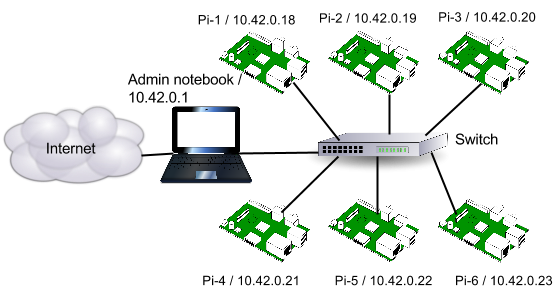
\includegraphics[scale=0.45]{png/pi_cluster.png} 
\centering
\caption{Subset of the testbed Cluster}
\end{figure}

The cluster is managed and controlled by a notebook. Additionally, we established a shared internet connection via the notbooks WiFi connection, allowing each host in the cluster to access the internet. 
By means of this network configuration we are able to run our Raspberry Pi cluster in the University network without the need to setup the internet connection for each host.

\paragraph{Deployment Software}
As already mentioned the \texttt{teda} distribution provides already some shell scripts to deploy erlang programs on multiple hosts in a network. We used the shell script \texttt{run\_dist.sh} as a starting point. To keep the report short we just sketch the implementaion of our testbed deployment software \texttt{venteda}.
We reimplemented the basic deployment steps in the previous mentioned shell script in a library called Venteda using the Ruby Programming Language. The different steps in the deployment process were implemented as separate functions.
The next figure shows the sequential workflow of the implemented deployment pipeline.
\begin{figure}[!htb]
\centering

\includegraphics[scale=0.5]{png/deployment_process.png}
\caption{Deployment pipeline} 
\end{figure}


For the sake of completeness the list below describes the implemeted deployment functions without going to much into the details.
\begin{itemize}
\itemsep0em
\item run() - launches an erlang application on the testbed 
\item read\_hosts() - reads a host file, specifies the hosts in the tesbed
\item package() - archives an application using tar
\item dsitribute() -  distributes a file on the testbed
\item upload\_file() - uploads a file using scp on a single host
\item unpack() - extracts the content of an archived application
\item start\_master() - starts the master erlang node
\item start\_nodes() - starts all erlang nodes

\end{itemize}

\section{Results}
\section{Conclusion}

As a final recommendation we would like to advocate for the use of Raspberry Pis in academia. They are great tool for learning how distributed systems work and they are very versatile, given you are not discouraged by the tinkering of the machines or the software that is required to get the most out of it's hardware.


\newpage
\addcontentsline{toc}{section}{References}
\bibliographystyle{plainnat}
\bibliography{biblio}
\nocite{*}


\end{document}
